% Options for packages loaded elsewhere
\PassOptionsToPackage{unicode}{hyperref}
\PassOptionsToPackage{hyphens}{url}
\PassOptionsToPackage{dvipsnames,svgnames,x11names}{xcolor}
\documentclass[
  10pt,
  fontset=fandol]{ctexart}
\usepackage{xcolor}
\usepackage[margin=16mm]{geometry}
\usepackage{amsmath,amssymb}
\setcounter{secnumdepth}{-\maxdimen} % remove section numbering
\usepackage{iftex}
\ifPDFTeX
  \usepackage[T1]{fontenc}
  \usepackage[utf8]{inputenc}
  \usepackage{textcomp} % provide euro and other symbols
\else % if luatex or xetex
  \usepackage{unicode-math} % this also loads fontspec
  \defaultfontfeatures{Scale=MatchLowercase}
  \defaultfontfeatures[\rmfamily]{Ligatures=TeX,Scale=1}
\fi
\usepackage{lmodern}
\ifPDFTeX\else
  % xetex/luatex font selection
\fi
% Use upquote if available, for straight quotes in verbatim environments
\IfFileExists{upquote.sty}{\usepackage{upquote}}{}
\IfFileExists{microtype.sty}{% use microtype if available
  \usepackage[]{microtype}
  \UseMicrotypeSet[protrusion]{basicmath} % disable protrusion for tt fonts
}{}
\makeatletter
\@ifundefined{KOMAClassName}{% if non-KOMA class
  \IfFileExists{parskip.sty}{%
    \usepackage{parskip}
  }{% else
    \setlength{\parindent}{0pt}
    \setlength{\parskip}{6pt plus 2pt minus 1pt}}
}{% if KOMA class
  \KOMAoptions{parskip=half}}
\makeatother
\usepackage{longtable,booktabs,array}
\newcounter{none} % for unnumbered tables
\usepackage{calc} % for calculating minipage widths
% Correct order of tables after \paragraph or \subparagraph
\usepackage{etoolbox}
\makeatletter
\patchcmd\longtable{\par}{\if@noskipsec\mbox{}\fi\par}{}{}
\makeatother
% Allow footnotes in longtable head/foot
\IfFileExists{footnotehyper.sty}{\usepackage{footnotehyper}}{\usepackage{footnote}}
\makesavenoteenv{longtable}
\usepackage{graphicx}
\makeatletter
\newsavebox\pandoc@box
\newcommand*\pandocbounded[1]{% scales image to fit in text height/width
  \sbox\pandoc@box{#1}%
  \Gscale@div\@tempa{\textheight}{\dimexpr\ht\pandoc@box+\dp\pandoc@box\relax}%
  \Gscale@div\@tempb{\linewidth}{\wd\pandoc@box}%
  \ifdim\@tempb\p@<\@tempa\p@\let\@tempa\@tempb\fi% select the smaller of both
  \ifdim\@tempa\p@<\p@\scalebox{\@tempa}{\usebox\pandoc@box}%
  \else\usebox{\pandoc@box}%
  \fi%
}
% Set default figure placement to htbp
\def\fps@figure{htbp}
\makeatother
\setlength{\emergencystretch}{3em} % prevent overfull lines
\providecommand{\tightlist}{%
  \setlength{\itemsep}{0pt}\setlength{\parskip}{0pt}}
\usepackage{amsmath,amssymb,mathtools,needspace}
\xeCJKDeclareCharClass{CJK}{"2032,"0400->"04FF,"2160->"216B,"2460->"2473,"25A0,"25C7,"25CB,"25CF}
\IfFontExistsTF{Arial Unicode MS}{\xeCJKsetup{AutoFallBack=true}\setCJKfallbackfamilyfont{\CJKrmdefault}{Arial Unicode MS}}{}
\setcounter{secnumdepth}{0}
\setlength{\emergencystretch}{2em}
\allowdisplaybreaks
\usepackage{bookmark}
\IfFileExists{xurl.sty}{\usepackage{xurl}}{} % add URL line breaks if available
\urlstyle{same}
\hypersetup{
  pdftitle={弦截法},
  colorlinks=true,
  linkcolor={Maroon},
  filecolor={Maroon},
  citecolor={Blue},
  urlcolor={Blue},
  pdfcreator={LaTeX via pandoc}}

\title{弦截法}
\author{}
\date{}

\begin{document}
\maketitle

\subsubsection{6.4.1 弦截法}\label{ux5f26ux622aux6cd5}

设 \(x_k,x_{k-1}\) 是 \(f(x)=0\) 的近似根，利用 \(f(x_k),f(x_{k-1})\) 构造一次插值多项式 \(P_1(x)\)，并用 \(P_1(x)=0\) 的根作为 \(f(x)=0\) 的新的近似根 \(x_{k+1}\)。由于

\[
P_1(x)=f(x_k)+\frac{f(x_k)-f(x_{k-1})}{x_k-x_{k-1}}(x-x_k),
\tag{6.4.1}
\]

因此有

\[
x_{k+1}=x_k-\frac{f(x_k)}{f(x_k)-f(x_{k-1})}(x_k-x_{k-1}).
\tag{6.4.2}
\]

这样导出的迭代公式（6.4.2）可以看作 Newton 公式 \(x_{k+1}=x_k-\dfrac{f(x_k)}{f'(x_k)}\) 中的导数 \(f'(x)\) 用差商 \(\dfrac{f(x_k)-f(x_{k-1})}{x_k-x_{k-1}}\) 取代的结果。

现在解释这种迭代过程的几何意义。如图 6.4 所示，曲线 \(y=f(x)\) 上横坐标为 \(x_k,x_{k-1}\) 的点分别记作 \(P_k,P_{k-1}\)，则弦线 \(P_kP_{k-1}\) 的斜率等于差商值 \(\dfrac{f(x_k)-f(x_{k-1})}{x_k-x_{k-1}}\)，其方程是

\[
f(x_k)+\frac{f(x_k)-f(x_{k-1})}{x_k-x_{k-1}}(x-x_k)=0.
\]

因此，按式（6.4.2）求得的 \(x_{k+1}\) 实际上是弦线 \(P_kP_{k-1}\) 与 \(x\) 轴交点的横坐标。这种算法因此而称为弦截法。

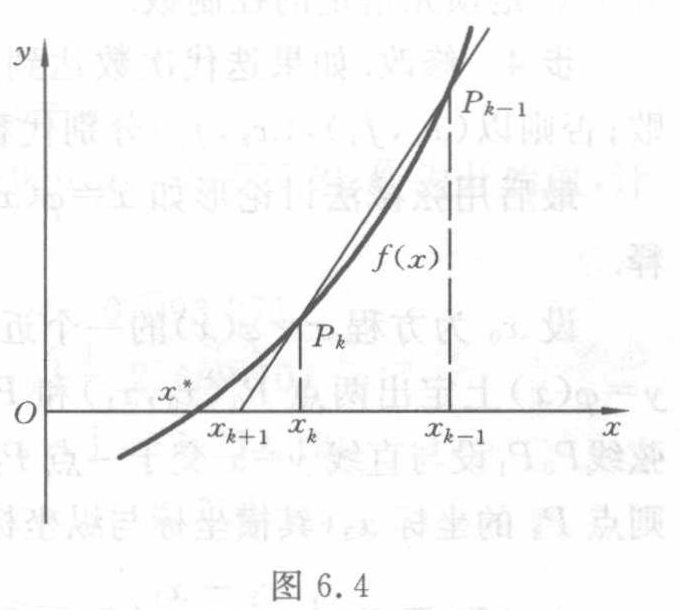
\includegraphics[width=0.85\linewidth,height=\textheight,keepaspectratio,alt={图 6.4 原扫描裁切}]{../assets/ch06/fig-6.4.png}

图 6.4

图意（agent 整理）：曲线上的 \(P_k,P_{k-1}\) 所连弦线与横轴交于横坐标 \(x_{k+1}\) 的点。全部标签为 \(x,\allowbreak y,\allowbreak O,\allowbreak x^*,\allowbreak x_{k+1},\allowbreak x_k,\allowbreak x_{k-1},\allowbreak P_k,\allowbreak P_{k-1},\allowbreak f(x)\)。

弦截法与切线法（Newton 法）都是线性化方法，但二者有本质的区别。切线法在计算 \(x_{k+1}\) 时只用到前一步的值 \(x_k\)，而弦截法（见式（6.4.2））在求 \(x_{k+1}\) 时要用到前面两步的结果 \(x_k,x_{k-1}\)，因此使用这种方法必须先给出两个开始值 \(x_0,x_1\)。

\textbf{例 6.9} 用弦截法解方程

\[
f(x)=x\mathrm{e}^x-1=0.
\]

\textbf{解} 设取 \(x_0=0.5,x_1=0.6\) 作为开始值，用弦截法求得的结果如表 6.9 所示，比较例 6.7 Newton 法的计算结果可以看出，弦截法的收敛速度也是相当快的。

表 6.9

{\def\LTcaptype{none} % do not increment counter
\begin{longtable}[]{@{}ll@{}}
\toprule\noalign{}
\(k\) & \(x_k\) \\
\midrule\noalign{}
\endhead
\bottomrule\noalign{}
\endlastfoot
\(0\) & \(0.5\) \\
\(1\) & \(0.6\) \\
\(2\) & \(0.565\,32\) \\
\(3\) & \(0.567\,09\) \\
\(4\) & \(0.567\,14\) \\
\end{longtable}
}

下述定理断言，弦截法具有超线性的收敛性。

\textbf{定理 6.4} 假设 \(f(x)\) 在根 \(x^*\) 的邻域 \(\Delta:|x-x^*|\leqslant\delta\) 内具有二阶连续导数，且对于任意

\begin{quote}
校注（agent 补充）：几何解释中原书称``其方程是''，随后印出的却是 \(P_1(x)=0\)，已照录。弦线本身的方程为 \(y=P_1(x)\)；原式表达的是弦线与 \(x\) 轴交点的条件，与随后求 \(x_{k+1}\) 的用途一致。
\end{quote}

\href{../../source-images/pdf-169.jpeg}{原页}

\(x\in\Delta\)，有 \(f'(x)\ne0\)，又初值 \(x_0,x_1\in\Delta\)，那么当邻域 \(\Delta\) 充分小时，弦截法（6.4.2）将按阶 \(p=\dfrac{1+\sqrt{5}}{2}\approx1.618\) 收敛到根 \(x^*\)。

由于定理 4 的证明比较烦琐，故略去不证。下面列出弦截法的计算步骤。

\textbf{步 1} 准备。选取初始近似值 \(x_0,x_1\)，计算相应的函数值 \(f_0=f(x_0),f_1=f(x_1)\)。

\textbf{步 2} 迭代。按公式

\[
x_2=x_1-f_1\bigg/\frac{f_1-f_0}{x_1-x_0}
\]

迭代一次得新的近似值 \(x_2\)，计算 \(f_2=f(x_2)\)。

\textbf{步 3} 控制。如果 \(x_2\) 满足 \(|\delta|\leqslant\varepsilon_1\) 或 \(|f_2|\leqslant\varepsilon_2\)，则认为过程收敛，终止迭代而以 \(x_2\) 作为所求的根；否则执行步 4。此处 \(\varepsilon_1,\varepsilon_2\) 是允许误差，而

\[
\delta=\begin{cases}
|x_2-x_1|,&\text{当 }|x_2|<C\text{ 时},\\
\dfrac{|x_2-x_1|}{|x_2|},&\text{当 }|x_2|\geqslant C\text{ 时},
\end{cases}
\]

其中 \(C\) 是预先指定的控制数。

\textbf{步 4} 修改。如果迭代次数达到预先指定的次数 \(N\)，则认为过程不收敛，计算失败；否则以 \((x_1,f_1),(x_2,f_2)\) 分别代替 \((x_0,f_0),(x_1,f_1)\)，而后转步 2 继续迭代。

最后用弦截法讨论形如 \(x=\varphi(x)\) 的方程，对 6.2.2 节的 Aitken 算法给出几何解释。

设 \(x_0\) 为方程 \(x=\varphi(x)\) 的一个近似根，依据迭代值 \(x_1=\varphi(x_0),x_2=\varphi(x_1)\) 在曲线 \(y=\varphi(x)\) 上定出两点 \(P_0(x_0,x_1)\) 和 \(P_1(x_1,x_2)\)，引弦线 \(P_0P_1\) 设与直线 \(y=x\) 交于一点 \(P_3\)（见图 6.5），则点 \(P_3\) 的坐标 \(x_3\)（其横坐标与纵坐标相等）满足

\[
x_3=x_1+\frac{x_2-x_1}{x_1-x_0}(x_3-x_0).
\]

由此解出

\[
x_3=\frac{x_0x_2-x_1^2}{x_0-2x_1+x_2},
\]

此即 Aitken 加速公式（6.2.2 节）。

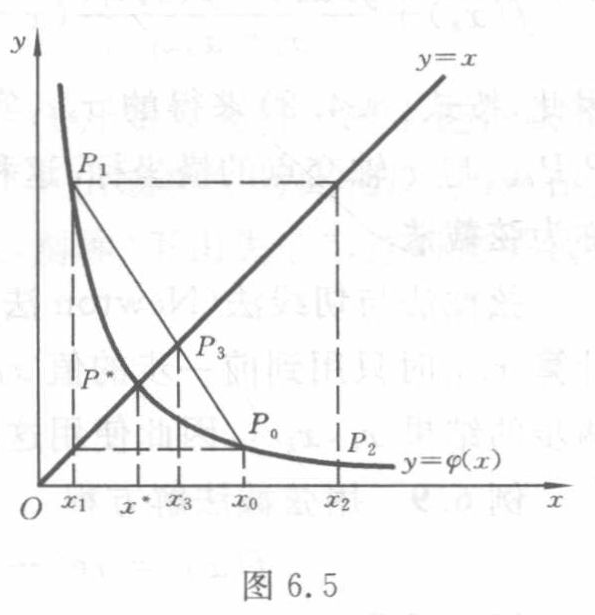
\includegraphics[width=0.85\linewidth,height=\textheight,keepaspectratio,alt={图 6.5 原扫描裁切}]{../assets/ch06/fig-6.5.png}

图 6.5

图意（agent 整理）：图用递减曲线 \(y=\varphi(x)\)、直线 \(y=x\)、弦线 \(P_0P_1\) 及其与 \(y=x\) 的交点 \(P_3\) 显示加速过程。全部标签为 \(x,\allowbreak y,\allowbreak O,\allowbreak x_1,\allowbreak x^*,\allowbreak x_3,\allowbreak x_0,\allowbreak x_2,\allowbreak P_1,\allowbreak P^*,\allowbreak P_3,\allowbreak P_0,\allowbreak P_2,\allowbreak y=x,\allowbreak y=\varphi(x)\)。

再考察图 6.5，所求的根 \(x^*\) 是曲线 \(y=\varphi(x)\) 与 \(y=x\) 交点 \(P^*\) 的横坐标，从图形上可以看出，尽管迭代值 \(x_2\) 比 \(x_0\) 和 \(x_1\) 更远地偏离了 \(x^*\)，但按上式定出的 \(x_3\) 却明显地扭转了这种发散的趋势。

\begin{center}\rule{0.5\linewidth}{0.5pt}\end{center}

\subsection{相关原页校注（agent 补充）}\label{ux76f8ux5173ux539fux9875ux6821ux6ce8agent-ux8865ux5145}

以下校注来自本节覆盖的原页，可能也涉及同页相邻小节；原文照录与校正说明分开保留。

\subsubsection{原书 PDF 页 169 的校注}\label{ux539fux4e66-pdf-ux9875-169-ux7684ux6821ux6ce8}

\href{../pages/pdf-169.md}{完整原页转录} · \href{../../source-images/pdf-169.jpeg}{原页图像}

校注记录：ch06-E010。

\begin{quote}
校注（agent 补充）：定理 6.4 的原文条件与 \(p=(1+\sqrt5)/2\) 结论均已保留。若将此处``按阶''理解为定义 6.2 中极限常数非零的精确收敛阶，还需 \(f''(x^*)\ne0\) 等非退化条件，并排除有限步已得根的情形。例如一次函数满足原定理的光滑性与导数非零条件，但弦截法可一步得根，不能一概赋予上述精确阶。
\end{quote}

\subsection{本节覆盖原页的校注记录}\label{ux672cux8282ux8986ux76d6ux539fux9875ux7684ux6821ux6ce8ux8bb0ux5f55}

下列记录按原页关联，含同页相邻小节的校注；计算时同时读取上文校注和完整原页。

\begin{itemize}
\tightlist
\item
  \texttt{ch06-E009}：原书 PDF 页 168
\item
  \texttt{ch06-E010}：原书 PDF 页 169
\end{itemize}

\end{document}
